% ============================================================================
%  COMPILE WITH XeLaTeX  (twice, so the point total resolves)
%  Overleaf: Menu -> Compiler -> XeLaTeX
%  Requires: bnhandout.sty and fonts/Kalpurush.ttf in the project
% ============================================================================
\documentclass[11pt]{article}
\usepackage{bnhandout}          % add [nosol] for a student edition

\hauthor[https://jugantordey.github.io]{Jugantor Dey}
\hseries{Mathematics for the Physics Olympiad}

\begin{document}

\handouttitle{Chapter 17 : Integration}

\noindent
এই অধ্যায়ের ভিত্তি ১৬ নম্বর অধ্যায়: $dy = f'(x)\,dx$, differential
আকারে chain rule, এবং $dm$, $dA$, $dV$ ধরনের ক্ষুদ্র উপাদান। ১৫ নম্বর
অধ্যায়ের derivative-এর তালিকাটি সারাক্ষণ হাতের কাছে লাগবে, আর ১৩ নম্বর
অধ্যায়ের অর্ধ কোণের সূত্রটি তৃতীয় অনুচ্ছেদে একবার লাগবে।

১৬ নম্বর অধ্যায় শেষ হয়েছিল একগুচ্ছ অসমাপ্ত বাক্য দিয়ে: দণ্ডের ভর, চাকতির
জড়তার ভ্রামক, গোলকের ভর, প্রতিটির জন্য $dm$ লেখা হয়েছিল আর বলা হয়েছিল ``যোগ
করার কাজটি ১৭ নম্বর অধ্যায়ের''। এই অধ্যায়ে সেই যোগগুলো করা হবে।

একটি কথা গোড়াতেই স্পষ্ট করে রাখা দরকার, কারণ প্রায় সব বইয়ে এটি উল্টো করে
শেখানো হয়। Integral-এর সংজ্ঞা ``derivative-এর উল্টো কাজ'' নয়। Integral হলো
অসংখ্য ক্ষুদ্র উপাদানের যোগফলের limit, একেবারে আলাদা একটি ধারণা, যার সঙ্গে
derivative-এর কোনো সম্পর্ক থাকার কথাই ছিল না। দুটি জিনিসকে যা একসঙ্গে বেঁধে
দেয় তার নাম Fundamental Theorem of Calculus, আর সেটি একটি \emph{উপপাদ্য},
সংজ্ঞা নয়। এই পার্থক্যটা ধরতে পারলে ক্যালকুলাসের অর্ধেক রহস্য কেটে যায়।

এই অধ্যায়ে মোট \totalpoints\ পয়েন্ট আছে।

\section{যোগফলের সীমা হিসেবে ইন্টিগ্রাল}

একটি বক্ররেখার নিচের ক্ষেত্রফল বের করতে চাই। আয়তক্ষেত্র বা ত্রিভুজের সূত্র
এখানে খাটে না, কারণ উপরের সীমানাটি সরল নয়। কিন্তু ১৪ নম্বর অধ্যায়ের
কৌশলটি খাটে: ছোট এলাকায় সবকিছু সরল।

তাই এলাকাটিকে সরু সরু আয়তক্ষেত্রে কেটে ফেলি, প্রতিটির ক্ষেত্রফল যোগ করি, তারপর
কাটার সংখ্যা বাড়াতে থাকি।

\begin{center}
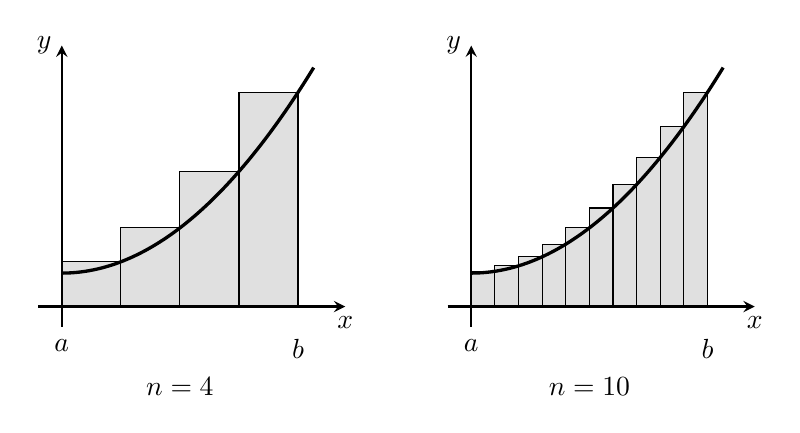
\begin{tikzpicture}[x=1.0cm,y=0.85cm,>=stealth]
 \begin{scope}
  \foreach \i in {0,1,2,3}{
    \pgfmathsetmacro\xl{\i*0.75}
    \pgfmathsetmacro\xr{(\i+1)*0.75}
    \pgfmathsetmacro\hh{0.3*\xr*\xr+0.5}
    \fill[black!12] (\xl,0) rectangle (\xr,\hh);
    \draw[thin] (\xl,0) rectangle (\xr,\hh);
  }
  \draw[thick,->] (-0.3,0) -- (3.6,0) node[below] {$x$};
  \draw[thick,->] (0,-0.3) -- (0,3.9) node[left] {$y$};
  \draw[very thick,domain=0:3.2,samples=80,variable=\x] plot ({\x},{0.3*\x*\x+0.5});
  \node[below] at (0,-0.35) {$a$};
  \node[below] at (3,-0.35) {$b$};
  \node at (1.5,-1.2) {$n=4$};
 \end{scope}
 \begin{scope}[xshift=5.2cm]
  \foreach \i in {0,...,9}{
    \pgfmathsetmacro\xl{\i*0.3}
    \pgfmathsetmacro\xr{(\i+1)*0.3}
    \pgfmathsetmacro\hh{0.3*\xr*\xr+0.5}
    \fill[black!12] (\xl,0) rectangle (\xr,\hh);
    \draw[thin] (\xl,0) rectangle (\xr,\hh);
  }
  \draw[thick,->] (-0.3,0) -- (3.6,0) node[below] {$x$};
  \draw[thick,->] (0,-0.3) -- (0,3.9) node[left] {$y$};
  \draw[very thick,domain=0:3.2,samples=80,variable=\x] plot ({\x},{0.3*\x*\x+0.5});
  \node[below] at (0,-0.35) {$a$};
  \node[below] at (3,-0.35) {$b$};
  \node at (1.5,-1.2) {$n=10$};
 \end{scope}
\end{tikzpicture}
\end{center}

\begin{idea}[Riemann sum ও নির্দিষ্ট integral]
$[a,b]$ ব্যবধিকে $n$টি সমান টুকরোয় ভাগ করো, প্রতিটির প্রস্থ
$\Delta x = \dfrac{b-a}{n}$। প্রতিটি টুকরো থেকে একটি নমুনা বিন্দু $x_{i}^{*}$
বেছে নিয়ে যোগফল তৈরি করো:
\[
  S_{n} = \sum_{i=1}^{n} f\left( x_{i}^{*} \right)\Delta x .
\]
একে বলে Riemann sum। এর limit-কে বলে নির্দিষ্ট integral:
\[
  \int_{a}^{b} f(x)\,dx = \lim_{n \to \infty} \sum_{i=1}^{n}
  f\left( x_{i}^{*} \right)\Delta x .
\]
\end{idea}

চিহ্নগুলো পড়ার নিয়মটা খেয়াল করো, কারণ তাতেই ধারণাটা লুকিয়ে আছে। $\int$
চিহ্নটি আসলে লম্বা করে টানা একটি S, অর্থাৎ ``sum''; $\sum$ চিহ্নটিরই উত্তরসূরি।
আর $dx$ হলো ১৬ নম্বর অধ্যায়ের তৃতীয় পাঠ: এক টুকরোর প্রস্থ। সব মিলিয়ে
$\int f\,dx$ পড়তে হয় ``$f\,dx$ ধরনের অসংখ্য ছোট অবদানের যোগফল''। ঠিক এই কারণেই
পদার্থবিজ্ঞানে $M = \int dm$ বা $I = \int r^{2}\,dm$ লেখা এত স্বাভাবিক।

দুটি কথা ধরে নেওয়া হচ্ছে, তাই বলে রাখি। এক, $f$ যদি $[a,b]$-তে continuous হয়,
তবে উপরের limit-টি সত্যিই থাকে। দুই, নমুনা বিন্দু $x_{i}^{*}$ কোথা থেকে বেছে
নেওয়া হলো (বাম প্রান্ত, ডান প্রান্ত, বা মাঝখান) তাতে limit বদলায় না। দুটোরই
প্রমাণ আছে, কিন্তু সেগুলো এই সিরিজের বাইরে; আমরা ধরে নিচ্ছি।

\begin{idea}[মৌলিক ধর্ম]
\[
  \int_{a}^{b}\left[ f + g \right]dx = \int_{a}^{b}f\,dx + \int_{a}^{b}g\,dx,
  \qquad
  \int_{a}^{b} cf\,dx = c\int_{a}^{b}f\,dx ,
\]
\[
  \int_{a}^{c}f\,dx + \int_{c}^{b}f\,dx = \int_{a}^{b}f\,dx, \qquad
  \int_{a}^{a}f\,dx = 0, \qquad
  \int_{b}^{a}f\,dx = -\int_{a}^{b}f\,dx .
\]
$[a,b]$-তে $f \leq g$ হলে $\int_{a}^{b}f\,dx \leq \int_{a}^{b}g\,dx$।
\end{idea}

প্রতিটিই Riemann sum-এর সংশ্লিষ্ট ধর্ম থেকে সরাসরি আসে, কারণ যোগফলের এই
ধর্মগুলো তো আমরা চিনিই; limit নিলেও তারা টেকে (১৪ নম্বর অধ্যায়ের limit-এর
নিয়ম)।

জ্যামিতিক অর্থ: $f \geq 0$ হলে $\int_{a}^{b}f\,dx$ হলো বক্ররেখার নিচের
ক্ষেত্রফল। $f$ ঋণাত্মক হলে ওই অংশের অবদান ঋণাত্মক, তাই সাধারণভাবে integral দেয়
\emph{চিহ্নযুক্ত} ক্ষেত্রফল।

\begin{example}
সংজ্ঞা থেকে $\int_{0}^{1} x\,dx$ নির্ণয় করো।
\end{example}

\begin{solbox}
$[0,1]$-কে $n$ টুকরোয় ভাগ করি, তাই $\Delta x = \dfrac{1}{n}$ এবং ডান প্রান্ত
নমুনা নিলে $x_{i}^{*} = \dfrac{i}{n}$। তখন
\[
  S_{n} = \sum_{i=1}^{n} \frac{i}{n} \cdot \frac{1}{n}
        = \frac{1}{n^{2}}\sum_{i=1}^{n} i
        = \frac{1}{n^{2}} \cdot \frac{n(n+1)}{2} ,
\]
যেখানে শেষ ধাপে ৮ নম্বর অধ্যায়ের যোগফল ব্যবহার করা হয়েছে। সরল করে
\[
  S_{n} = \frac{n+1}{2n} = \frac{1}{2} + \frac{1}{2n} .
\]
$n \to \infty$-এ এটি $\dfrac{1}{2}$-এ যায়, সুতরাং
\[
  \int_{0}^{1} x\,dx = \frac{1}{2} .
\]
যাচাই: এলাকাটি একটি সমকোণী ত্রিভুজ, ভূমি $1$ ও উচ্চতা $1$, ক্ষেত্রফল
$\tfrac{1}{2}$। মিলে গেল।

এবং এখানেই সমস্যাটা স্পষ্ট: এত সহজ একটি integral বের করতেই ধারার যোগফলের সূত্র
লাগল। $\int_{0}^{1}\sin x\,dx$ এভাবে করতে গেলে কী হতো ভাবো। পরের অনুচ্ছেদই
এর সমাধান।
\end{solbox}

\prob{2} $\int_{0}^{2} x^{2}\,dx$-এর মান চারটি সমান টুকরো ও ডান প্রান্ত নমুনা
নিয়ে আসন্নভাবে বের করো। প্রকৃত মান $\dfrac{8}{3}$; তোমার উত্তর বেশি না কম
এল, এবং কেন?

\begin{sol}
$\Delta x = 0.5$ এবং ডান প্রান্তগুলো $0.5, 1, 1.5, 2$। সুতরাং
\[
  S_{4} = \left( 0.25 + 1 + 2.25 + 4 \right) \times 0.5 = 7.5 \times 0.5
  = 3.75 .
\]
প্রকৃত মান $\dfrac{8}{3} \approx 2.667$, তাই আসন্ন মানটি বেশি।

কারণ: $[0,2]$-তে $x^{2}$ বর্ধমান, তাই প্রতিটি টুকরোয় ডান প্রান্তের মানই
সবচেয়ে বড়। ফলে প্রতিটি আয়তক্ষেত্র বক্ররেখার উপরে বেরিয়ে যায় এবং যোগফল
অতিরিক্ত হয়। বাম প্রান্ত নিলে উল্টোটা হতো।
\end{sol}

\prob{3} সংজ্ঞা থেকে $\int_{0}^{b} x\,dx = \dfrac{b^{2}}{2}$ প্রমাণ করো
($b > 0$)।

\begin{sol}
$\Delta x = \dfrac{b}{n}$ এবং ডান প্রান্ত $x_{i}^{*} = \dfrac{ib}{n}$। তাই
\[
  S_{n} = \sum_{i=1}^{n} \frac{ib}{n} \cdot \frac{b}{n}
        = \frac{b^{2}}{n^{2}}\sum_{i=1}^{n} i
        = \frac{b^{2}}{n^{2}} \cdot \frac{n(n+1)}{2}
        = \frac{b^{2}}{2}\left( 1 + \frac{1}{n} \right) .
\]
$n \to \infty$-এ $\dfrac{1}{n} \to 0$, সুতরাং limit $\dfrac{b^{2}}{2}$।

জ্যামিতিক যাচাই: ভূমি $b$ ও উচ্চতা $b$-এর সমকোণী ত্রিভুজ, ক্ষেত্রফল
$\tfrac{1}{2}b^{2}$।
\end{sol}

\prob{2} $\int_{0}^{3}f = 5$ এবং $\int_{0}^{1}f = 2$ দেওয়া আছে।
\begin{enumerate}
  \item $\int_{1}^{3}f$ নির্ণয় করো।
  \item $\int_{3}^{0}f$ নির্ণয় করো।
  \item কোনো হিসাব না করে $\int_{-2}^{2} x^{3}\,dx$-এর মান বলো এবং কারণ দাও।
\end{enumerate}

\begin{sol}
\begin{enumerate}
  \item ব্যবধি জোড়ার ধর্ম থেকে $\int_{0}^{1} + \int_{1}^{3} =
        \int_{0}^{3}$, তাই $\int_{1}^{3}f = 5 - 2 = 3$।
  \item সীমা উল্টালে চিহ্ন উল্টায়, তাই $\int_{3}^{0}f = -5$।
  \item $x^{3}$ একটি অড ফাংশন (১০ নম্বর অধ্যায়), আর ব্যবধিটি
        মূলবিন্দু সাপেক্ষে প্রতিসম। বাম অর্ধেকের চিহ্নযুক্ত ক্ষেত্রফল ডান
        অর্ধেকের ঠিক ঋণাত্মক, তাই যোগফল শূন্য: $\int_{-2}^{2}x^{3}dx = 0$।
\end{enumerate}
তৃতীয়টিই ১০ নম্বর অধ্যায়ে প্রতিসাম্য নিয়ে যে কথাটি বলা হয়েছিল তার
নির্ভুল রূপ।
\end{sol}

\section{মৌলিক উপপাদ্য (Fundamental Theorem of Calculus)}

Riemann sum দিয়ে প্রতিটি integral বের করা অসম্ভব। ভাগ্য ভালো, দরকার নেই।

\begin{idea}[মৌলিক উপপাদ্য, প্রথম অংশ]
$f$ যদি $[a,b]$-তে continuous হয় এবং
\[
  F(x) = \int_{a}^{x} f(t)\,dt ,
\]
তবে $F$ differentiable এবং $F'(x) = f(x)$।
\end{idea}

\begin{center}
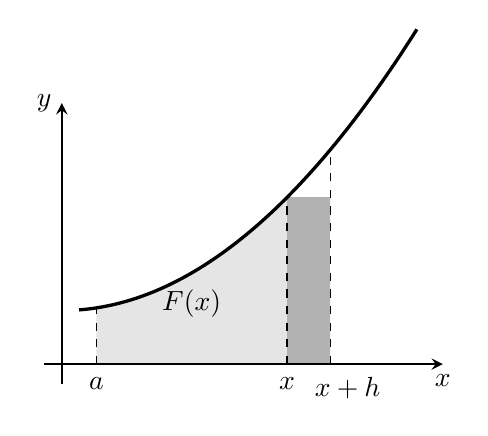
\begin{tikzpicture}[x=1.1cm,y=0.85cm,>=stealth]
  \fill[black!10,domain=0.4:2.6,samples=60,variable=\x]
     plot ({\x},{0.25*\x*\x+0.8}) -- (2.6,0) -- (0.4,0) -- cycle;
  \fill[black!30] (2.6,0) rectangle (3.1,2.49);
  \draw[thick,->] (-0.2,0) -- (4.4,0) node[below] {$x$};
  \draw[thick,->] (0,-0.3) -- (0,3.9) node[left] {$y$};
  \draw[very thick,domain=0.2:4.1,samples=80,variable=\x] plot ({\x},{0.25*\x*\x+0.8});
  \draw[dashed] (0.4,0) -- (0.4,0.84);
  \draw[dashed] (2.6,0) -- (2.6,2.49);
  \draw[dashed] (3.1,0) -- (3.1,3.20);
  \node[below] at (0.4,-0.05) {$a$};
  \node[below] at (2.6,-0.05) {$x$};
  \node[below] at (3.3,-0.05) {$x+h$};
  \node at (1.5,0.9) {$F(x)$};
\end{tikzpicture}
\end{center}

প্রমাণটি ছবিতেই আছে। $F(x+h) - F(x)$ হলো $x$ থেকে $x+h$ পর্যন্ত সরু ফালিটির
ক্ষেত্রফল, অর্থাৎ
\[
  F(x+h) - F(x) = \int_{x}^{x+h} f(t)\,dt .
\]
ওই ছোট ব্যবধিতে $f$-এর সর্বনিম্ন মান $m$ এবং সর্বোচ্চ মান $M$ ধরি। ফালিটি
$m$ উচ্চতার আয়তক্ষেত্রের চেয়ে বড় এবং $M$ উচ্চতারটির চেয়ে ছোট, তাই
\[
  m\,h \leq F(x+h) - F(x) \leq M\,h .
\]
$h$ দিয়ে ভাগ করে
\[
  m \leq \frac{F(x+h)-F(x)}{h} \leq M .
\]
এবার $h \to 0$ নাও। ব্যবধিটি ছোট হতে হতে $x$ বিন্দুতে গুটিয়ে আসে, আর $f$
continuous বলে $m$ ও $M$ দুটিই $f(x)$-এর দিকে যায়। Squeeze Theorem
(১৪ নম্বর অধ্যায়) অনুযায়ী মাঝেরটিও $f(x)$-এ যায়, অর্থাৎ $F'(x) = f(x)$।

(এখানে ধরে নেওয়া হয়েছে যে বদ্ধ ব্যবধিতে continuous ফাংশনের সর্বনিম্ন ও
সর্বোচ্চ মান সত্যিই থাকে। এটি একটি উপপাদ্য, যার প্রমাণ ১৪ নম্বর অধ্যায়ের
Intermediate Value Theorem-এর মতোই বাস্তব সংখ্যার গভীর ধর্মের উপর দাঁড়ানো;
আমরা ধরে নিচ্ছি।)

\begin{idea}[মৌলিক উপপাদ্য, দ্বিতীয় অংশ]
$f$ continuous এবং $F$ যদি $f$-এর যেকোনো একটি antiderivative হয় (অর্থাৎ
$F' = f$), তবে
\[
  \int_{a}^{b} f(x)\,dx = F(b) - F(a) .
\]
\end{idea}

প্রথম অংশ থেকে দ্বিতীয়টি বেরিয়ে আসে। $G(x) = \int_{a}^{x}f$ ধরো; প্রথম অংশ
বলছে $G' = f$। তাহলে $(F-G)' = 0$, আর যে ফাংশনের derivative সর্বত্র শূন্য সে
ধ্রুবক (এই ফলটির প্রমাণে Mean Value Theorem লাগে, যা ১৫ নম্বর অধ্যায়ের
মতোই এখানেও ধরে নেওয়া হচ্ছে)। সুতরাং $F = G + C$, এবং
\[
  F(b) - F(a) = \left[ G(b)+C \right] - \left[ G(a)+C \right]
  = G(b) - G(a) = \int_{a}^{b}f.
\]

\begin{remark}
এখানে থেমে একবার ভাবো, কারণ ব্যাপারটা সত্যিই আশ্চর্যের। বাম পাশে আছে অসংখ্য
সরু ফালির যোগফলের limit, যা এলাকার গোটা আকৃতির উপর নির্ভর করে। ডান পাশে আছে
কেবল দুটি বিন্দুতে একটি ফাংশনের মান। মাঝখানের সব তথ্য কোথায় গেল? Integral আর
derivative যে একে অপরের বিপরীত কাজ, এই সত্যটিই ওই তথ্যটুকু বহন করছে। এটি
সংজ্ঞা দিয়ে পাওয়া যায় না, প্রমাণ করে আদায় করতে হয়; সেজন্যই এর নাম
উপপাদ্য।
\end{remark}

Antiderivative-এর সেটকে লেখা হয় নির্দিষ্ট সীমা ছাড়া, যাকে বলে অনির্দিষ্ট
integral:
\[
  \int f(x)\,dx = F(x) + C .
\]
ধ্রুবক $C$ বাদ দেওয়া যায় না, কারণ যেকোনো ধ্রুবক যোগ করলেও derivative একই
থাকে। ১৫ নম্বর অধ্যায়ের derivative-এর তালিকাটি উল্টো দিক থেকে পড়লেই
নিচের তালিকাটি পাওয়া যায়।

\begin{center}
\begin{tabular}{c|c}
 $f(x)$ & $\int f(x)\,dx$ \\ \hline
 $x^{n}$ ($n \neq -1$) & $\dfrac{x^{n+1}}{n+1} + C$ \\[1mm]
 $\dfrac{1}{x}$ & $\ln|x| + C$ \\[1mm]
 $e^{x}$ & $e^{x} + C$ \\[1mm]
 $\sin x$ & $-\cos x + C$ \\[1mm]
 $\cos x$ & $\sin x + C$ \\[1mm]
 $\dfrac{1}{\cos^{2}x}$ & $\tan x + C$ \\
\end{tabular}
\end{center}

$\dfrac{1}{x}$-এর ঘরে পরম মান চিহ্নটি খেয়াল করো: $x<0$-এও সূত্রটি খাটে, কারণ
$\dfrac{d}{dx}\ln(-x) = \dfrac{-1}{-x} = \dfrac{1}{x}$।

\begin{example}
১৬ নম্বর অধ্যায়ের দণ্ডটির হিসাব শেষ করো: $x = 0$ থেকে $L$ পর্যন্ত
$\lambda(x) = \lambda_{0}\left( 1 + \dfrac{x}{L} \right)$ হলে মোট ভর কত?
\end{example}

\begin{solbox}
সেখানে পাওয়া গিয়েছিল $dm = \lambda_{0}\left( 1 + \dfrac{x}{L} \right)dx$।
এখন কেবল যোগ করতে হবে, অর্থাৎ $x$-কে $0$ থেকে $L$ পর্যন্ত চালাতে হবে:
\[
  M = \int dm = \int_{0}^{L}\lambda_{0}\left( 1 + \frac{x}{L} \right)dx
    = \lambda_{0}\left[ x + \frac{x^{2}}{2L} \right]_{0}^{L}
    = \lambda_{0}\left( L + \frac{L}{2} \right) = \frac{3\lambda_{0}L}{2} .
\]
যাচাই: ঘনত্ব $\lambda_{0}$ থেকে $2\lambda_{0}$ পর্যন্ত সরলরৈখিকভাবে বাড়ে, তাই
গড় ঘনত্ব $\tfrac{3}{2}\lambda_{0}$ এবং ভর $\tfrac{3}{2}\lambda_{0}L$। মিলে
গেল।
\end{solbox}

\prob{2} নির্ণয় করো।
\begin{enumerate}
  \item $\int_{1}^{4}\left( 3x^{2} - 2x + 1 \right)dx$
  \item $\int_{0}^{\pi} \sin x\,dx$
  \item $\int_{1}^{e} \dfrac{dx}{x}$
\end{enumerate}

\begin{sol}
\begin{enumerate}
  \item Antiderivative $x^{3} - x^{2} + x$, তাই মান
        $(64-16+4) - (1-1+1) = 52 - 1 = 51$।
  \item $\left[ -\cos x \right]_{0}^{\pi} = -(-1) - (-1) = 2$।
  \item $\left[ \ln x \right]_{1}^{e} = 1 - 0 = 1$।
\end{enumerate}
\end{sol}

\prob{2} নির্ণয় করো।
\begin{enumerate}
  \item $\dfrac{d}{dx}\displaystyle\int_{0}^{x}\sin\left( t^{2} \right)dt$
  \item $\dfrac{d}{dx}\displaystyle\int_{0}^{x^{2}} e^{-t}\,dt$
\end{enumerate}

\begin{sol}
\begin{enumerate}
  \item মৌলিক উপপাদ্যের প্রথম অংশ সরাসরি দেয় $\sin\left( x^{2} \right)$।
        খেয়াল করো, $\sin(t^{2})$-এর কোনো সরল antiderivative নেই, তবু
        derivative-টা বের করা গেল।
  \item এখানে উপরের সীমা $x$ নয়, $x^{2}$। তাই
        $G(u) = \int_{0}^{u}e^{-t}dt$ ধরে chain rule প্রয়োগ করি:
        \[
          \frac{d}{dx}G\left( x^{2} \right) = G'\left( x^{2} \right)\cdot 2x
          = e^{-x^{2}} \cdot 2x .
        \]
\end{enumerate}
\end{sol}

\prob{3} ১৬ নম্বর অধ্যায়ের দণ্ডটির জন্য ($\lambda = \lambda_{0}(1+x/L)$)
ভরকেন্দ্রের অবস্থান $\bar{x} = \dfrac{\int x\,dm}{\int dm}$ নির্ণয় করো।

\begin{sol}
হর আগেই পাওয়া গেছে: $\int dm = \dfrac{3\lambda_{0}L}{2}$।

লব:
\[
  \int x\,dm = \int_{0}^{L}\lambda_{0}\left( x + \frac{x^{2}}{L} \right)dx
  = \lambda_{0}\left[ \frac{x^{2}}{2} + \frac{x^{3}}{3L} \right]_{0}^{L}
  = \lambda_{0}\left( \frac{L^{2}}{2} + \frac{L^{2}}{3} \right)
  = \frac{5\lambda_{0}L^{2}}{6} .
\]
সুতরাং
\[
  \bar{x} = \frac{5\lambda_{0}L^{2}/6}{3\lambda_{0}L/2} = \frac{5L}{9} .
\]
যাচাই: $\dfrac{5}{9} \approx 0.56$, অর্থাৎ মাঝবিন্দুর সামান্য ডানে। ঘনত্ব
ডান দিকে বেশি, তাই ভরকেন্দ্র ডানে সরে যাওয়াই স্বাভাবিক।
\end{sol}

\prob{3} ১৫ নম্বর অধ্যায়ের কণাটির বেগ $v(t) = 3t^{2} - 12t + 9$।
\begin{enumerate}
  \item $t = 0$ থেকে $t = 3$ পর্যন্ত সরণ নির্ণয় করো।
  \item একই সময়ে অতিক্রান্ত মোট দূরত্ব নির্ণয় করো।
\end{enumerate}

\begin{sol}
\begin{enumerate}
  \item সরণ $= \int_{0}^{3}v\,dt = \left[ t^{3}-6t^{2}+9t \right]_{0}^{3}
        = 27 - 54 + 27 = 0$।
  \item দূরত্ব $= \int_{0}^{3}|v|\,dt$, তাই আগে চিহ্ন দেখতে হবে।
        $v = 3(t-1)(t-3)$, অর্থাৎ $0<t<1$-এ $v>0$ এবং $1<t<3$-এ $v<0$।
        \[
          \int_{0}^{1}v\,dt = 1 - 6 + 9 = 4, \qquad
          \int_{1}^{3}v\,dt = 0 - 4 = -4 .
        \]
        সুতরাং মোট দূরত্ব $4 + |-4| = 8$।
\end{enumerate}
সরণ শূন্য অথচ দূরত্ব আট: কণাটি ৪ একক এগিয়ে গিয়ে ৪ একক ফিরে এসেছে। চিহ্ন
আলাদা না করে $\int v\,dt$ নিলে দূরত্বের প্রশ্নের ভুল উত্তর আসত।
\end{sol}

\section{কৌশল}

Antiderivative খুঁজে বের করার কোনো যান্ত্রিক পদ্ধতি নেই; derivative নেওয়ার
যেমন আছে, তেমন নয়। কিন্তু তিনটি কৌশল বেশিরভাগ কাজ সেরে দেয়, আর তিনটিই ১৫ ও
১৬ নম্বর অধ্যায়ের নিয়ম উল্টো দিক থেকে পড়ে পাওয়া।

\begin{idea}[প্রতিস্থাপন (Substitution)]
$u = g(x)$ ধরলে $du = g'(x)\,dx$, এবং
\[
  \int f\bigl( g(x) \bigr)g'(x)\,dx = \int f(u)\,du .
\]
নির্দিষ্ট integral-এ সীমাগুলোও বদলাতে হয়: $x = a$-এর জায়গায় $u = g(a)$।
\end{idea}

এটি chain rule-এরই উল্টো পাঠ। ১৬ নম্বর অধ্যায়ে বলা হয়েছিল যে differential
আকারে $du$ একটি সত্যিকারের রাশি, তাই তাকে যান্ত্রিকভাবে বসিয়ে দেওয়া বৈধ; এই
কৌশলটিই তার সরাসরি ফল।

\begin{idea}[অংশে অংশে যোগজীকরণ (Integration by parts)]
Product rule বলে $d(uv) = u\,dv + v\,du$। দুই পাশে যোগ করে সাজালে
\[
  \int u\,dv = uv - \int v\,du .
\]
\end{idea}

কৌশলটা হলো integrand-কে $u$ ও $dv$-তে এমনভাবে ভাগ করা যাতে নতুন integral-টি
পুরনোটির চেয়ে সহজ হয়। সাধারণ নিয়ম: যাকে derivative নিলে সরল হয় তাকে $u$
বানাও ($x$, $x^{2}$, $\ln x$), আর যাকে integrate করা সহজ তাকে $dv$
($e^{x}dx$, $\sin x\,dx$)।

\begin{idea}[আংশিক ভগ্নাংশ]
$a \neq b$ হলে
\[
  \frac{1}{(x-a)(x-b)} = \frac{1}{a-b}\left( \frac{1}{x-a}
  - \frac{1}{x-b} \right) ,
\]
আর ডান পাশের প্রতিটি পদ আলাদা করে integrate করা যায়।
\end{idea}

সমীকরণটি যাচাই করা সহজ: ডান পাশ এক ভগ্নাংশে আনলে লব দাঁড়ায়
$\dfrac{(x-b)-(x-a)}{a-b} = 1$। এখানে কেবল আলাদা একঘাতী গুণনীয়কের ক্ষেত্রটি
দেখানো হলো; পুনরাবৃত্ত বা দ্বিঘাত গুণনীয়ক থাকলে পদ্ধতিটি একই থাকে, কেবল
বীজগণিতটা লম্বা হয় (এসব ক্ষেত্রে কীভাবে আংশিক ভগ্নাংশ বের করতে হয় তার নিয়মগুলো নবম-দশম শ্রেণির উচ্চতর গণিত বিষয়ের বইয়ে পাবে)।

\begin{example}
নির্ণয় করো: (ক) $\int 2x\sqrt{1+x^{2}}\,dx$; (খ) $\int x\cos x\,dx$;
(গ) $\int_{0}^{2\pi}\sin^{2}x\,dx$।
\end{example}

\begin{solbox}
(ক) $u = 1+x^{2}$ ধরি, তাই $du = 2x\,dx$ এবং integrand হয়ে যায়
$\sqrt{u}\,du$:
\[
  \int u^{1/2}\,du = \frac{2}{3}u^{3/2} + C
  = \frac{2}{3}\left( 1+x^{2} \right)^{3/2} + C .
\]

(খ) $u = x$ ও $dv = \cos x\,dx$ নিই, তাই $du = dx$ ও $v = \sin x$:
\[
  \int x\cos x\,dx = x\sin x - \int \sin x\,dx = x\sin x + \cos x + C .
\]
উল্টো ভাগ করলে ($u = \cos x$) নতুন integral-টি আরও কঠিন হতো; ভাগটা বেছে নেওয়াই
এখানে আসল কাজ।

(গ) সরাসরি antiderivative নেই, তাই আগে ১৩ নম্বর অধ্যায়ের অর্ধ কোণের সূত্র
ব্যবহার করি: $\sin^{2}x = \dfrac{1-\cos 2x}{2}$। তখন
\[
  \int_{0}^{2\pi}\sin^{2}x\,dx
  = \frac{1}{2}\int_{0}^{2\pi}dx - \frac{1}{2}\int_{0}^{2\pi}\cos 2x\,dx
  = \frac{1}{2}(2\pi) - \frac{1}{2}\left[ \frac{\sin 2x}{2} \right]_{0}^{2\pi}
  = \pi .
\]
ফলটি মনে রাখার মতো: এক পূর্ণ চক্রে $\sin^{2}$-এর গড় মান ঠিক $\tfrac{1}{2}$।
পর্যাবৃত্ত গতি ও তরঙ্গের গড় শক্তির হিসাবে এটি বারবার লাগে।
\end{solbox}

\prob{2} প্রতিস্থাপন ব্যবহার করে নির্ণয় করো।
\begin{enumerate}
  \item $\int 2x\left( 1+x^{2} \right)^{4}dx$
  \item $\int \sin x\cos^{2}x\,dx$
  \item $\int_{0}^{1} x e^{x^{2}}\,dx$
\end{enumerate}

\begin{sol}
\begin{enumerate}
  \item $u = 1+x^{2}$, $du = 2x\,dx$, তাই
        $\int u^{4}du = \dfrac{u^{5}}{5}+C
        = \dfrac{\left( 1+x^{2} \right)^{5}}{5}+C$।
  \item $u = \cos x$, $du = -\sin x\,dx$, তাই
        $-\int u^{2}du = -\dfrac{u^{3}}{3}+C = -\dfrac{\cos^{3}x}{3}+C$।
  \item $u = x^{2}$, $du = 2x\,dx$; সীমা বদলায় $x=0 \to u=0$ এবং
        $x=1 \to u=1$:
        \[
          \frac{1}{2}\int_{0}^{1}e^{u}du = \frac{1}{2}\left( e - 1 \right) .
        \]
\end{enumerate}
\end{sol}

\prob{2} অংশে অংশে যোগজীকরণ ব্যবহার করে নির্ণয় করো।
\begin{enumerate}
  \item $\int x e^{x}\,dx$
  \item $\int x\sin x\,dx$
  \item $\int \ln x\,dx$
\end{enumerate}

\begin{sol}
\begin{enumerate}
  \item $u = x$, $dv = e^{x}dx$: $xe^{x} - \int e^{x}dx = (x-1)e^{x}+C$।
  \item $u = x$, $dv = \sin x\,dx$, তাই $v = -\cos x$:
        $-x\cos x + \int\cos x\,dx = -x\cos x + \sin x + C$।
  \item কৌশল: $u = \ln x$ এবং $dv = dx$ নাও, তাই $du = \dfrac{dx}{x}$ ও
        $v = x$:
        \[
          \int \ln x\,dx = x\ln x - \int x \cdot \frac{dx}{x}
          = x\ln x - x + C .
        \]
        যাচাই: derivative নিলে $\ln x + 1 - 1 = \ln x$।
\end{enumerate}
\end{sol}

\prob{3} $\int x^{2}e^{x}\,dx$ নির্ণয় করো।

\begin{sol}
$u = x^{2}$, $dv = e^{x}dx$:
\[
  \int x^{2}e^{x}dx = x^{2}e^{x} - 2\int xe^{x}dx .
\]
ডান পাশের integral-টি উপরের সমস্যায় পাওয়া গেছে, $(x-1)e^{x}$। সুতরাং
\[
  \int x^{2}e^{x}dx = x^{2}e^{x} - 2(x-1)e^{x} + C
  = \left( x^{2}-2x+2 \right)e^{x} + C .
\]
যাচাই: derivative নিলে $(2x-2)e^{x} + (x^{2}-2x+2)e^{x} = x^{2}e^{x}$।

সাধারণ নিয়ম: $x^{n}e^{x}$ ধরনের integral-এ $n$ বার অংশে অংশে প্রয়োগ করলে
ঘাত এক এক করে নেমে শূন্যে পৌঁছায়।
\end{sol}

\prob{3} নির্ণয় করো।
\begin{enumerate}
  \item $\displaystyle\int \frac{dx}{(x-1)(x+3)}$
  \item $\displaystyle\int_{0}^{1} \frac{dx}{(x+1)(x+2)}$
\end{enumerate}

\begin{sol}
\begin{enumerate}
  \item $a = 1$, $b = -3$, তাই $a - b = 4$ এবং
        \[
          \frac{1}{(x-1)(x+3)}
          = \frac{1}{4}\left( \frac{1}{x-1} - \frac{1}{x+3} \right) .
        \]
        Integrate করে
        \[
          \frac{1}{4}\left( \ln|x-1| - \ln|x+3| \right) + C
          = \frac{1}{4}\ln\left| \frac{x-1}{x+3} \right| + C .
        \]
  \item $a = -1$, $b = -2$, তাই $a-b = 1$ এবং
        $\dfrac{1}{(x+1)(x+2)} = \dfrac{1}{x+1} - \dfrac{1}{x+2}$। সুতরাং
        \[
          \int_{0}^{1} = \left[ \ln\frac{x+1}{x+2} \right]_{0}^{1}
          = \ln\frac{2}{3} - \ln\frac{1}{2}
          = \ln\frac{4}{3} \approx 0.2877 .
        \]
\end{enumerate}
\end{sol}

\section{বক্ররেখার দৈর্ঘ্য}

এবার ১৬ নম্বর অধ্যায়ের কায়দাটি নতুন একটি রাশিতে প্রয়োগ করি। প্রশ্ন:
একটি বাঁকা রেখার দৈর্ঘ্য কত?

কৌশল সেই একই। বক্ররেখাটিকে অসংখ্য ছোট টুকরোয় ভাগ করো; প্রতিটি টুকরো এত ছোট যে
তাকে সরলরেখা ধরা যায়; তারপর যোগ করো।

\begin{center}
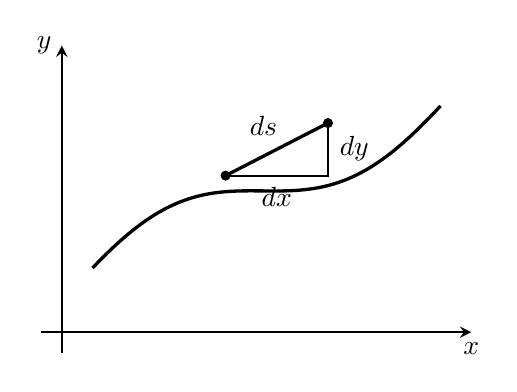
\begin{tikzpicture}[x=1.3cm,y=1.3cm,>=stealth]
  \draw[thick,->] (-0.2,0) -- (4.0,0) node[below] {$x$};
  \draw[thick,->] (0,-0.2) -- (0,2.8) node[left] {$y$};
  \draw[very thick,domain=0.3:3.7,samples=80,variable=\x] plot ({\x},{0.55*\x+0.35*sin(1.6*\x r)+0.3});
  \draw[thick] (1.6,1.529) -- (2.6,1.529) -- (2.6,2.043);
  \draw[very thick] (1.6,1.529) -- (2.6,2.043);
  \draw[fill] (1.6,1.529) circle (1.6pt);
  \draw[fill] (2.6,2.043) circle (1.6pt);
  \node[below] at (2.1,1.51) {$dx$};
  \node[right] at (2.62,1.79) {$dy$};
  \node[above left] at (2.2,1.83) {$ds$};
\end{tikzpicture}
\end{center}

\begin{idea}[চাপের উপাদান]
\[
  ds = \sqrt{dx^{2} + dy^{2}}
     = \sqrt{1 + \left( \frac{dy}{dx} \right)^{2}}\;dx ,
\]
এবং $x = a$ থেকে $x = b$ পর্যন্ত বক্ররেখার দৈর্ঘ্য
\[
  s = \int_{a}^{b}\sqrt{1 + \left( \frac{dy}{dx} \right)^{2}}\;dx .
\]
Polar স্থানাঙ্কে বাহু দুটি $dr$ ও $r\,d\theta$ (১৬ নম্বর অধ্যায়), তাই
\[
  ds = \sqrt{dr^{2} + r^{2}d\theta^{2}}
     = \sqrt{\left( \frac{dr}{d\theta} \right)^{2} + r^{2}}\;d\theta .
\]
\end{idea}

যুক্তিটা ছবির সমকোণী ত্রিভুজটিই: অনুভূমিক বাহু $dx$, উল্লম্ব বাহু $dy$, আর
কর্ণ $ds$; Pythagoras প্রয়োগ করলেই প্রথম সমীকরণ। দ্বিতীয় রূপটি পাওয়া যায়
বর্গমূলের ভেতর থেকে $dx^{2}$ বের করে এনে।


\begin{example}
$y = \tfrac{2}{3}x^{3/2}$ বক্ররেখার $x=0$ থেকে $x=3$ পর্যন্ত দৈর্ঘ্য নির্ণয়
করো।
\end{example}

\begin{solbox}
$\dfrac{dy}{dx} = x^{1/2}$, তাই $1 + \left( \dfrac{dy}{dx} \right)^{2}
= 1 + x$ এবং
\[
  s = \int_{0}^{3}\sqrt{1+x}\;dx
    = \left[ \frac{2}{3}(1+x)^{3/2} \right]_{0}^{3}
    = \frac{2}{3}\left( 8 - 1 \right) = \frac{14}{3} \approx 4.67 .
\]
যাচাই: বক্ররেখার দুই প্রান্ত $(0,0)$ ও $(3, 2\sqrt{3}) \approx (3, 3.46)$, আর
তাদের সরলরৈখিক দূরত্ব $\sqrt{9+12} \approx 4.58$। বাঁকা পথ সরল পথের চেয়ে
সামান্য বড়, ঠিক যেমন হওয়া উচিত।
\end{solbox}

\prob{2} $y = \dfrac{x^{3}}{3} + \dfrac{1}{4x}$ বক্ররেখার $x=1$ থেকে $x=2$
পর্যন্ত দৈর্ঘ্য নির্ণয় করো।

\begin{sol}
\[
  \frac{dy}{dx} = x^{2} - \frac{1}{4x^{2}} .
\]
বর্গ করে $1$ যোগ করি:
\[
  1 + \left( x^{2} - \frac{1}{4x^{2}} \right)^{2}
  = 1 + x^{4} - \frac{1}{2} + \frac{1}{16x^{4}}
  = x^{4} + \frac{1}{2} + \frac{1}{16x^{4}}
  = \left( x^{2} + \frac{1}{4x^{2}} \right)^{2} .
\]
পূর্ণবর্গ হয়ে গেল, তাই বর্গমূল নেওয়া সহজ:
\[
  s = \int_{1}^{2}\left( x^{2} + \frac{1}{4x^{2}} \right)dx
    = \left[ \frac{x^{3}}{3} - \frac{1}{4x} \right]_{1}^{2}
    = \left( \frac{8}{3} - \frac{1}{8} \right)
      - \left( \frac{1}{3} - \frac{1}{4} \right)
    = \frac{59}{24} \approx 2.46 .
\]
বইয়ের চাপের দৈর্ঘ্যের সমস্যাগুলো প্রায় সবসময়ই এভাবে সাজানো থাকে যাতে
বর্গমূলের ভেতরটা পূর্ণবর্গ হয়; নইলে integral-টি সাধারণত হাতে করা যায় না।
\end{sol}

\prob{3} লগারিদমীয় সর্পিল (logarithmic spiral) $r = a e^{k\theta}$ ($a, k > 0$)।
\begin{enumerate}
  \item $ds$ নির্ণয় করো।
  \item $\theta = 0$ থেকে $\theta = \Theta$ পর্যন্ত দৈর্ঘ্য নির্ণয় করো।
\end{enumerate}

\begin{sol}
\begin{enumerate}
  \item $\dfrac{dr}{d\theta} = ake^{k\theta} = kr$, তাই
        \[
          ds = \sqrt{(kr)^{2} + r^{2}}\;d\theta
             = r\sqrt{1+k^{2}}\;d\theta
             = a\sqrt{1+k^{2}}\;e^{k\theta}d\theta .
        \]
  \item \[
          s = a\sqrt{1+k^{2}}\int_{0}^{\Theta}e^{k\theta}d\theta
            = \frac{a\sqrt{1+k^{2}}}{k}\left( e^{k\Theta} - 1 \right) .
        \]
\end{enumerate}
লক্ষ করো, উত্তরটি $\dfrac{\sqrt{1+k^{2}}}{k}$ গুণ ($r$-এর বৃদ্ধি), অর্থাৎ
দৈর্ঘ্য ব্যাসার্ধের সমানুপাতিক। এই কারণেই লগারিদমীয় সর্পিলকে বলা হয়
স্ব-সদৃশ: যত বড় করেই দেখো, আকৃতি একই থাকে।
\end{sol}

\prob{3} শিকল-বক্ররেখা (catenary) $y = a\cosh\dfrac{x}{a}$, যেখানে
$\cosh u = \dfrac{e^{u}+e^{-u}}{2}$ এবং $\sinh u = \dfrac{e^{u}-e^{-u}}{2}$
(১০ নম্বর অধ্যায়)।
\begin{enumerate}
  \item দেখাও যে $\dfrac{d}{du}\cosh u = \sinh u$।
  \item $x = 0$ থেকে $x = b$ পর্যন্ত দৈর্ঘ্য নির্ণয় করো।
\end{enumerate}

\begin{sol}
\begin{enumerate}
  \item সংজ্ঞা থেকে সরাসরি:
        \[
          \frac{d}{du}\cdot\frac{e^{u}+e^{-u}}{2}
          = \frac{e^{u}-e^{-u}}{2} = \sinh u .
        \]
  \item Chain rule প্রয়োগ করে $\dfrac{dy}{dx} = \sinh\dfrac{x}{a}$। ১০ নম্বর
        অধ্যায়ে প্রমাণিত হয়েছিল $\cosh^{2}u - \sinh^{2}u = 1$, তাই
        \[
          1 + \sinh^{2}\frac{x}{a} = \cosh^{2}\frac{x}{a} ,
        \]
        এবং $\cosh > 0$ বলে বর্গমূল নিলে $\cosh\dfrac{x}{a}$। সুতরাং
        \[
          s = \int_{0}^{b}\cosh\frac{x}{a}\,dx
            = \left[ a\sinh\frac{x}{a} \right]_{0}^{b}
            = a\sinh\frac{b}{a} .
        \]
\end{enumerate}
ঝুলন্ত তার বা শিকল ঠিক এই আকৃতি নেয়, আর সেটিই এর নামের কারণ। এখানে বর্গমূলের
ভেতরটা আবার পূর্ণবর্গ হয়ে গেল, এবার একটি অভেদের কল্যাণে।
\end{sol}

\section{ক্ষেত্রফল ও আয়তন}

\begin{idea}[দুটি বক্ররেখার মধ্যবর্তী ক্ষেত্রফল]
$[a,b]$-তে $f \geq g$ হলে তাদের মধ্যবর্তী ক্ষেত্রফল
\[
  A = \int_{a}^{b}\left[ f(x) - g(x) \right]dx .
\]
\end{idea}

উপাদানটি ভাবো একটি সরু উল্লম্ব ফালি হিসেবে: প্রস্থ $dx$, উচ্চতা $f-g$, তাই
$dA = (f-g)\,dx$।

\begin{idea}[ফালি করে আয়তন (Volumes by slicing)]
কোনো ঘনবস্তুকে $x$-অক্ষের লম্বভাবে কাটলে যদি প্রস্থচ্ছেদের ক্ষেত্রফল $A(x)$
হয়, তবে
\[
  V = \int_{a}^{b}A(x)\,dx .
\]
বিশেষ ক্ষেত্র: $y = f(x)$ বক্ররেখাকে $x$-অক্ষের চারদিকে ঘোরালে প্রস্থচ্ছেদ
একটি চাকতি, তাই
\[
  V = \int_{a}^{b}\pi\left[ f(x) \right]^{2}dx .
\]
\end{idea}

এখানে থেমে একবার পেছনে তাকাও। ১১ নম্বর অধ্যায়ে গোলক ও cone-এর আয়তন বের
করা হয়েছিল ``প্রতিটি উচ্চতায় প্রস্থচ্ছেদ সমান হলে আয়তনও সমান'' এই নীতিটি
ধরে নিয়ে, আর বলা হয়েছিল যে ১৭ নম্বর অধ্যায়ে এটি এক লাইনে বেরিয়ে আসবে।
উপরের সমীকরণটিই সেই এক লাইন।

\begin{example}
চাকতি পদ্ধতি ব্যবহার করে $R$ ব্যাসার্ধের গোলকের আয়তন নির্ণয় করো।
\end{example}

\begin{solbox}
\begin{center}
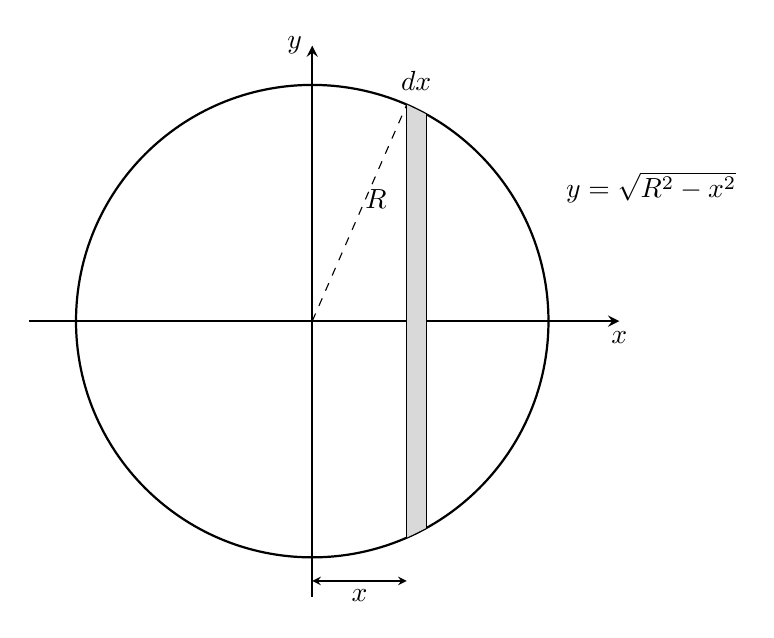
\begin{tikzpicture}[x=1.0cm,y=1.0cm,>=stealth]
  \draw[thick,->] (-3.6,0) -- (3.9,0) node[below] {$x$};
  \draw[thick,->] (0,-3.5) -- (0,3.5) node[left] {$y$};
  \draw[thick] (0,0) circle (3);
  \fill[black!15] (1.2,-2.749) -- (1.2,2.749) -- (1.45,2.626) -- (1.45,-2.626) -- cycle;
  \draw[thin] (1.2,-2.749) -- (1.2,2.749);
  \draw[thin] (1.45,-2.626) -- (1.45,2.626);
  \draw[dashed] (0,0) -- (1.2,2.749);
  \node[above right] at (0.55,1.3) {$R$};
  \draw[<->] (0,-3.3) -- (1.2,-3.3);
  \node[below] at (0.6,-3.28) {$x$};
  \node[right] at (3.1,1.7) {$y=\sqrt{R^{2}-x^{2}}$};
  \node[above] at (1.32,2.80) {$dx$};
\end{tikzpicture}
\end{center}

গোলকটিকে ভাবো $y = \sqrt{R^{2}-x^{2}}$ অর্ধবৃত্তকে $x$-অক্ষের চারদিকে ঘুরিয়ে
পাওয়া। $x$ অবস্থানে চাকতিটির ব্যাসার্ধ $\sqrt{R^{2}-x^{2}}$, তাই
\[
  dV = \pi\left( R^{2}-x^{2} \right)dx .
\]
এখন $x$-কে $-R$ থেকে $R$ পর্যন্ত চালাই:
\[
  V = \pi\int_{-R}^{R}\left( R^{2}-x^{2} \right)dx
    = \pi\left[ R^{2}x - \frac{x^{3}}{3} \right]_{-R}^{R}
    = \pi\left[ \left( R^{3}-\frac{R^{3}}{3} \right)
      - \left( -R^{3}+\frac{R^{3}}{3} \right) \right] .
\]
বন্ধনী খুলে
\[
  V = \pi \cdot \frac{4R^{3}}{3} = \frac{4}{3}\pi R^{3} .
\]
১১ নম্বর অধ্যায়ে এই ফলটি প্রস্থচ্ছেদের নীতি ধরে নিয়ে পাওয়া গিয়েছিল; এবার
সেটি হিসাব করেই পাওয়া গেল।
\end{solbox}

\prob{2} $y = x^{2}$ ও $y = x$ বক্ররেখা দুটির মধ্যবর্তী ক্ষেত্রফল নির্ণয় করো।

\begin{sol}
ছেদবিন্দু: $x^{2} = x$ দেয় $x = 0$ ও $x = 1$। ওই ব্যবধিতে $x \geq x^{2}$
(যেমন $x = 0.5$-এ $0.5 > 0.25$), তাই উপরের বক্ররেখা $y = x$। সুতরাং
\[
  A = \int_{0}^{1}\left( x - x^{2} \right)dx
    = \left[ \frac{x^{2}}{2} - \frac{x^{3}}{3} \right]_{0}^{1}
    = \frac{1}{2} - \frac{1}{3} = \frac{1}{6} .
\]
\end{sol}

\prob{3} চাকতি পদ্ধতি ব্যবহার করে $r$ ব্যাসার্ধ ও $h$ উচ্চতার cone-এর আয়তন
নির্ণয় করো, এবং ১১ নম্বর অধ্যায়ের ফলের সঙ্গে মেলাও।

\begin{sol}
Cone-টিকে ভাবো $x$-অক্ষ বরাবর শোয়ানো, শীর্ষবিন্দু মূলবিন্দুতে এবং ভূমি
$x = h$-এ। তখন ঘূর্ণিত রেখাটি $y = \dfrac{r}{h}x$, কারণ $x=0$-এ ব্যাসার্ধ শূন্য
এবং $x=h$-এ $r$।

$x$ অবস্থানে চাকতির ব্যাসার্ধ $\dfrac{rx}{h}$, তাই
\[
  dV = \pi\frac{r^{2}x^{2}}{h^{2}}\,dx ,
\]
এবং
\[
  V = \frac{\pi r^{2}}{h^{2}}\int_{0}^{h}x^{2}dx
    = \frac{\pi r^{2}}{h^{2}} \cdot \frac{h^{3}}{3}
    = \frac{1}{3}\pi r^{2}h .
\]
১১ নম্বর অধ্যায়ে ঘনককে তিনটি pyramid-এ কেটে এবং প্রস্থচ্ছেদের নীতি ধরে
নিয়ে একই $\tfrac{1}{3}$ পাওয়া গিয়েছিল। সেখানে যা ধরে নিতে হয়েছিল, এখানে
তা প্রমাণ হলো।
\end{sol}

\prob{3} ১৬ নম্বর অধ্যায়ের চাকতির হিসাব শেষ করো। $R$ ব্যাসার্ধের একটি
সমসত্ত্ব চাকতির পৃষ্ঠ ঘনত্ব $\sigma$। কেন্দ্র দিয়ে যাওয়া লম্ব অক্ষের সাপেক্ষে
তার জড়তার ভ্রামক $I$ নির্ণয় করো এবং $M$-এর মাধ্যমে প্রকাশ করো।

\begin{sol}
প্রতিসাম্য কাজে লাগাই: $\theta$-এর উপর কিছুই নির্ভর করে না, তাই $\theta$
বরাবর আগেই যোগ করে ফেলা যায় এবং উপাদান হিসেবে গোটা একটি সরু বৃত্তাকার বলয়
নেওয়া যায়। $r$ ব্যাসার্ধের বলয়ের পরিধি $2\pi r$ ও প্রস্থ $dr$, তাই
\[
  dA = 2\pi r\,dr, \qquad dm = 2\pi\sigma r\,dr, \qquad
  dI = r^{2}dm = 2\pi\sigma r^{3}dr .
\]
যোগ করি:
\[
  I = 2\pi\sigma\int_{0}^{R}r^{3}dr = 2\pi\sigma \cdot \frac{R^{4}}{4}
    = \frac{\pi\sigma R^{4}}{2} .
\]
মোট ভর $M = \sigma \pi R^{2}$, তাই $\pi\sigma = \dfrac{M}{R^{2}}$ এবং
\[
  I = \frac{1}{2}MR^{2} .
\]
১৬ নম্বর অধ্যায়ে যে উত্তরটির কথা বলা হয়েছিল, সেটিই পাওয়া গেল।
\end{sol}

\prob{4} ১৬ নম্বর অধ্যায়ের গোলকটির হিসাব শেষ করো। $R$ ব্যাসার্ধের নিরেট
গোলকের ঘনত্ব $\rho(r) = \rho_{0}\left( 1 - \dfrac{r}{R} \right)$, এবং সেখানে
পাওয়া গিয়েছিল
\[
  dm = 4\pi\rho_{0}\left( 1-\frac{r}{R} \right)r^{2}dr, \qquad
  dI = \frac{8\pi\rho_{0}}{3}\left( 1-\frac{r}{R} \right)r^{4}dr .
\]
\begin{enumerate}
  \item মোট ভর $M$ নির্ণয় করো।
  \item জড়তার ভ্রামক $I$ নির্ণয় করো এবং $MR^{2}$-এর গুণিতক হিসেবে লেখো।
  \item সমসত্ত্ব গোলকের জন্য $I = \tfrac{2}{5}MR^{2}$। তোমার উত্তরটি এর
        চেয়ে বড় না ছোট, এবং কেন?
\end{enumerate}

\begin{sol}
\begin{enumerate}
  \item \[
          M = 4\pi\rho_{0}\int_{0}^{R}\left( r^{2} - \frac{r^{3}}{R} \right)dr
            = 4\pi\rho_{0}\left[ \frac{R^{3}}{3} - \frac{R^{3}}{4} \right]
            = 4\pi\rho_{0}\cdot\frac{R^{3}}{12}
            = \frac{\pi\rho_{0}R^{3}}{3} .
        \]
  \item \[
          I = \frac{8\pi\rho_{0}}{3}\int_{0}^{R}
              \left( r^{4} - \frac{r^{5}}{R} \right)dr
            = \frac{8\pi\rho_{0}}{3}\left[ \frac{R^{5}}{5}
              - \frac{R^{5}}{6} \right]
            = \frac{8\pi\rho_{0}}{3}\cdot\frac{R^{5}}{30}
            = \frac{4\pi\rho_{0}R^{5}}{45} .
        \]
        প্রথম অংশ থেকে $\pi\rho_{0} = \dfrac{3M}{R^{3}}$, তাই
        \[
          I = \frac{4R^{5}}{45}\cdot\frac{3M}{R^{3}} = \frac{4}{15}MR^{2} .
        \]
  \item $\dfrac{4}{15} \approx 0.267$, আর $\dfrac{2}{5} = 0.4$; সুতরাং
        আমাদের উত্তরটি ছোট।

        কারণ: এই গোলকে ঘনত্ব কেন্দ্রে সবচেয়ে বেশি এবং পৃষ্ঠে শূন্য, অর্থাৎ
        ভরের বেশিরভাগ অক্ষের কাছে জমা। জড়তার ভ্রামকে দূরত্ব বর্গ হয়ে ঢোকে,
        তাই কাছে জমা ভর কম অবদান রাখে। ভেতরের দিকে ভর সরানো মানেই $I$ কমা।
\end{enumerate}
\end{sol}

\end{document}
